
\subsection{Implementado un Event-Handler}

En el contexto de Smart Campus UIS, cada uno de los mensajes enviados por los dispositivos es manejado como un evento. Es decir, cada mensaje recibido debe ser registrado y procesado por los microservicios de administración para lograr un objetivo final. Este procesamiento, recuerda al patrón de diseño \textit{Observer} en el cual se busca el realizar una acción cada vez que el estado, de lo que se está observando, cambia \cite{Shvets2019}.

Siendo así, se estableció el realizar la implementación de un observador el cual se hará responsable de la captura de los mensajes enviados por los dispositivos y establecer el estado del sistema. De esto, como se puede ver en la figura \ref{fig:proceso_looker} se propuso un proceso que debía realizar el observador a implementar.

\begin{figure}[ht]
    \caption{Primera propuesta del proceso a realizar \linebreak por el observador a implementar} 
    \centering
    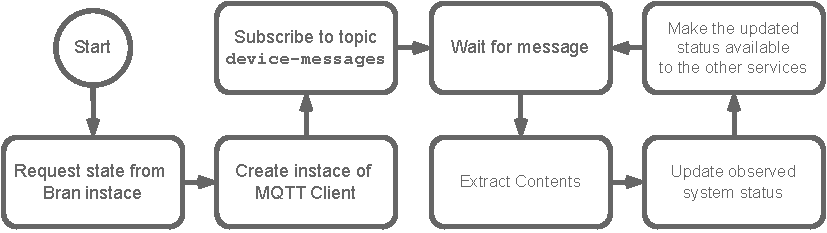
\includegraphics[width=\linewidth]{images/LookerProcess.pdf}
    \label{fig:proceso_looker}
\end{figure} 

Este primer acercamiento, es bastante directo en cuanto a la implementación a realizar. Esta se basa en la inicialización de un cliente de MQTT, subscrito al tópico usado por los dispositivos conectados a Smart Campus, \texttt{device-messages}, \cite{SmartCampusGithub}, y procesar cada uno de los mensajes a medida que estos van llegando. 

En este primer prototipo del observador, existen algunas limitaciones a resolver. El primero de estas que no le da acceso al observador, de aquí en adelante referido como \textit{Looker}, acceder al contexto geográfico, requerido para evaluar el estado de cada una de las locaciones de la aplicación. 

Esto se solucionó realizando una petición de la descripción del campus, requerido para la declaración del estado objetivo, a un endpoint que tenga estos datos. Para su implementación fue necesario realizar una modificación a \textit{Lexical} para que este, tras validar la arquitectura objetivo, envíe el resultado serializado a un servicio encargado de almacenar las arquitecturas objetivo. 

Así mismo, quedaba por definir el cómo el resto de los tendrían acceso al estado actualizado de la aplicación. Esto se implementó de dos maneras. La primera es con un endpoint HTTP en el cual se puede 

% 
De la misma manera, quedaba pendiente el definir el como los demás servicios podrán acceder a los datos que están siendo procesados. Es decir, si vamos a usar un bus de datos para publicar el estado del sistema al resto de los servicios, o permitir el acceso con peticiones HTTP a través de un endpoint.

% 
La implementación de esto depende del como se desee realizar el manejo de los cambios en la arquitectura de Smart Campus UIS. Si se desea responder de manera inmediata a cambios en la arquitectura, se tendría que usar un bus de datos, como MQTT o AMQP; pero tendría la consecuencia de un aumento en el uso de los recursos debido a que se tendrían que procesar todos los cambios cada vez que se determine el estado de la aplicación. 

% 
En el caso contrario, podría implementarse un endpoint HTTP el cual sea consultado en intervalos de tiempo por el servicio encargado de comparar los estados objetivo y de referencia. Esto permitiría tener un mayor control de cada cuanto se realizan las comparaciones, y más importante, cada cuanto se realizan acciones sobre la arquitectura actual con el fin de modificarla hacia el estado de referencia.

Siendo así, y debido a querer manejar más el control desde el servicio encargado de los cambios en la arquitectura, que se escogió la opción de emplear un endpoint. De esta manera, se podrá regular cada cuanto se realizan acciones sobre Smart Campus UIS, lo que debería resultar en un comportamiento más predecible.

Finalmente, este primer prototipo, no establece el como se realizará la evaluación del estado del sistema. De no tener una métrica la cual evaluar, no se habrá manera de detectar las diferentes alteraciones al estado actual del sistema.

Para esto, del contexto proveído, se tomaron las propiedades con el fin de establecer el estado de un componente. Ahora, a pesar de considerar otros parámetros y puntos de medida para el servicio, debido a la gran cantidad de necesidades que pudiera presentar un usuario final, como lo pueden ser el mantener datos en un rango o la distribución entre estos; se decidió, para efectos de esta implementación inicial, sólo tomar como parámetros básicos el tiempo entre mensajes de los dispositivos y la cantidad de estos en una locación. La nueva estructura del proyecto, hasta el momento, puede observarse en la figura \ref{fig:StarDuckBasic}.
 
% Esta primera parte se solucionó realizando una petición de la descripción del campus, requerido para la declaración del estado objetivo, a un endpoint que tenga estos datos. Para su implementación fue necesario realizar una modificación a Lexical para que este, tras validar la arquitectura objetivo, envíe el resultado serializado a un servicio encargado de almacenar las arquitecturas objetivo. La nueva estructura del proyecto, hasta el momento, puede observarse en la figura \ref{fig:StarDuckBasic}.

\begin{figure}[ht]
    \centering
    \caption{Arquitectura actual del proyecto}
    \label{fig:StarDuckBasic}
    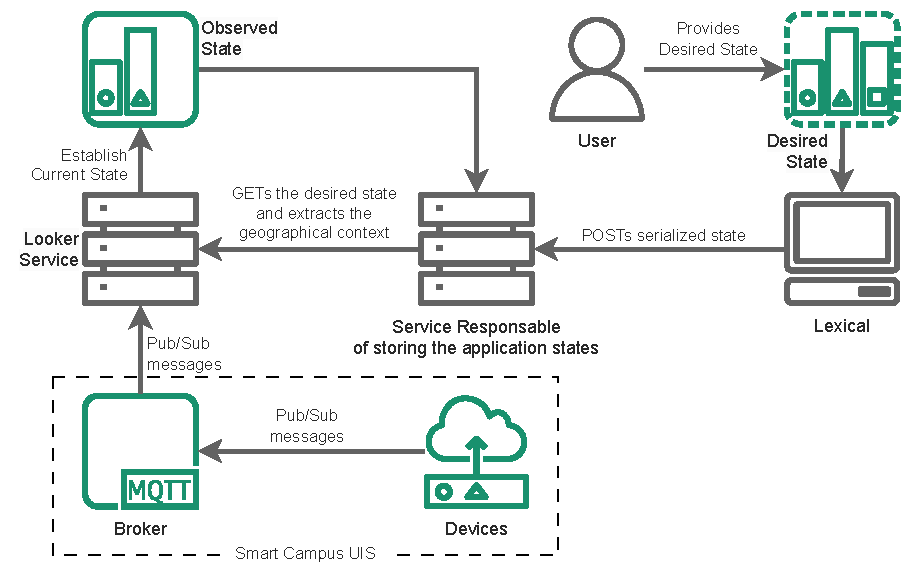
\includegraphics[width=\linewidth]{images/StarDuckBasic.pdf}
\end{figure}

% Respecto al segundo punto, la implementación de este depende del como se desee realizar el manejo de los cambios en la arquitectura de Smart Campus UIS. Si se desea responder de manera inmediata a cambios en la arquitectura, se tendría que usar un bus de datos, como MQTT o AMQP; pero tendría la consecuencia de un aumento en el uso de los recursos debido a que se tendrían que procesar todos los cambios cada vez que se determine el estado de la aplicación. 

% En el caso contrario, podría implementarse un endpoint HTTP el cual sea consultado en intervalos de tiempo por el servicio encargado de comparar los estados objetivo y de referencia. Esto permitiría tener un mayor control de cada cuanto se realizan las comparaciones, y más importante, cada cuanto se realizan acciones sobre la arquitectura actual con el fin de modificarla hacia el estado de referencia.

% Siendo así, y debido a querer manejar más el control desde el servicio encargado de los cambios en la arquitectura, que se escogió la opción de emplear un endpoint. De esta manera, se podrá regular cada cuanto se realizan acciones sobre Smart Campus UIS, lo que debería resultar en un comportamiento más predecible.

% Ahora, en cuanto a la manera en la que se evaluará el estado de los diferentes orígenes de datos. Para esto, del contexto proveído, se tomaron las propiedades con el fin de establecer el estado de un componente. Ahora, a pesar de considerar otros parámetros y puntos de medida para nuestro servicio, debido a la gran cantidad de necesidades que pudiera presentar un usuario final, como lo pueden ser el mantener datos en un rango o la distribución entre estos; se decidió, para efectos de esta implementación inicial, sólo tomar como parámetros básicos el tiempo entre mensajes de los dispositivos y la cantidad de estos en una locación. 